\chapter{Venerable Venerables}

Earlier I mentioned that, during the period of my first visit back to
New Zealand after having left Thailand, it quickly became evident that
we were faced with the task of not just translating texts, but also of
translating traditions. In the meditation monasteries in North East
Thailand, there was more or less one way of doing things which we simply
adopted, or at least tried hard to adopt; sometimes we didn't quite
succeed, to the amusement of our hosts. Now, in this new context, we
were discovering that we had to learn how to accord with the ways things
were done in Bangkok, Cambodia, Laos, Vietnam, Sri Lanka, Burma, and of
course, Britain. Buddhism had been here for
a significant period of time\cite{uk-buddhism}
and British Buddhists already had certain assumptions and expectations.

Occasionally, as mentioned earlier, during those initial years at
Chithurst, someone would suggest that it was time to start thinking
about changing this or that way of doing things. Ajahn Sumedho was slow
to engage such proposals, and appeared to derive strength from his
commitment to honouring the way of doing things that we had been taught
during those formative years in Thailand.

One issue, though, that really did capture the interest of most of us,
was the possibility of changing the dates for the period of the annual
Rains Retreat. In India two and a half thousand years ago, the Buddha
instructed the sangha that they should cease from wandering during the
three months of the monsoon season; this roughly coincides these days
with July, August and September. Inconsiderate monks had caused
annoyance to the laypeople by trampling their paddy fields, and besides,
a regular period each year of more focussed formal practice was useful.
In Britain, however, that period of the year was when the weather was
mild and actually more suitable for travelling around. It was also a
better time of year for doing outdoor maintenance work; it was not an
ideal time for formal retreating. Try as they might, however, those with
a good understanding of the monastic code of discipline were not able to
find any suitable way of making an adjustment; the \emph{Vinaya} simply
didn't allow for it. So it was accepted that we would find ways to live
with that structure as it was.

Tempering our excessive eagerness to change structures to suit our
preferences is no different from restraining the hyperactive mind in
meditation. If we call it a problem, then we have to deal with the
consequences of having created a problem. In reality there are no
problems. In reality there are difficulties, pain and irritation, but
problems are something extra we create out of the resistance which is an
expression of unawareness.

The benefits that stem from living in harmonious community are
considerable and it behoves us to regularly reflect on that. Community
is the container. Because of that container, the heat and pressure that
inevitably builds up as we progress in spiritual practice, is made more
manageable. It is not insignificant that the Buddha identified community
(sangha) as one of the Three Refuges. The consequences of messing with
community structures might not always be obvious, and by the time we do
come around to seeing any consequences, it could be too late, as the
cohesive element of concord might already have been lost. Sometimes I
ponder on the process of a caterpillar transforming into a butterfly,
and the function of the chrysalis. The caterpillar is obvious and we are
fascinated looking at it; the butterfly is obvious and beautiful; but
how much value do we place on that which serves as the `container'
during that process of transformation? The container deserves a lot of
care and attention.

It was a boon in those early years to often receive visits from senior
sangha members. Sometimes without warning, an elder from Sri Lanka or
Burma might turn up. Presumably they wanted to see what these Westerners
were doing; and, as far as I recall, it was always the case that they
wanted to be helpful.

Their sage advice gave us confidence and, I think it is true enough to
say, moderated some of our excessive enthusiasm. Whatever clever ideas
we might have about \emph{Dhamma-Vinaya}, or insights we thought we had
experienced, there is no substitute for the benefit that comes from
years of experience. There is a unique beauty to be found in maturity.

Venerable Ananda Maitreya\cite{ananda}
from Sri Lanka visited us several times over
the years. There is one particularly lovely memory I have of an occasion
when he was staying and the Venerable Taungpulu Sayadaw\cite{taungpulu}
from Burma arrived. Both were in their
nineties at the time, I believe, and it was a joy to witness the
interaction between these two elders. It is customary, when monks meet
each other for the first time, that they respectfully enquire as to
which year they had taken up the monks' Precepts. Although Ven. Ananda
Maitreya knew many languages, Burmese was not one of them; the only
language they had in common was Pali. It then transpired that they had
both taken up the training in the same year, so the conversation
proceeded to which month. Once that was established, the junior of the
two bowed to the senior. I feel tears welling up even now thinking about
it. Besides the beauty that can come with maturity, there is also the
admiration one feels on witnessing such commitment and endurance. This
is the beauty of virtue. In Dhammapada verse 55 the Buddha comments,

\begin{quote}
  The fragrance of virtue surpasses by far\\
  the fragrance of flowers or sandalwood.
\end{quote}

Possibly due to the way the early translators of the traditional
Theravada Buddhist texts render the Pali word \emph{Bhante}, these days
in Britain, even very junior Buddhist monks are addressed as Venerable.
I have occasionally attempted to dissuade people from using the word
venerable in that way, but with little success. In my opinion it would
be good if the word could be reserved for actually venerable
Venerables.

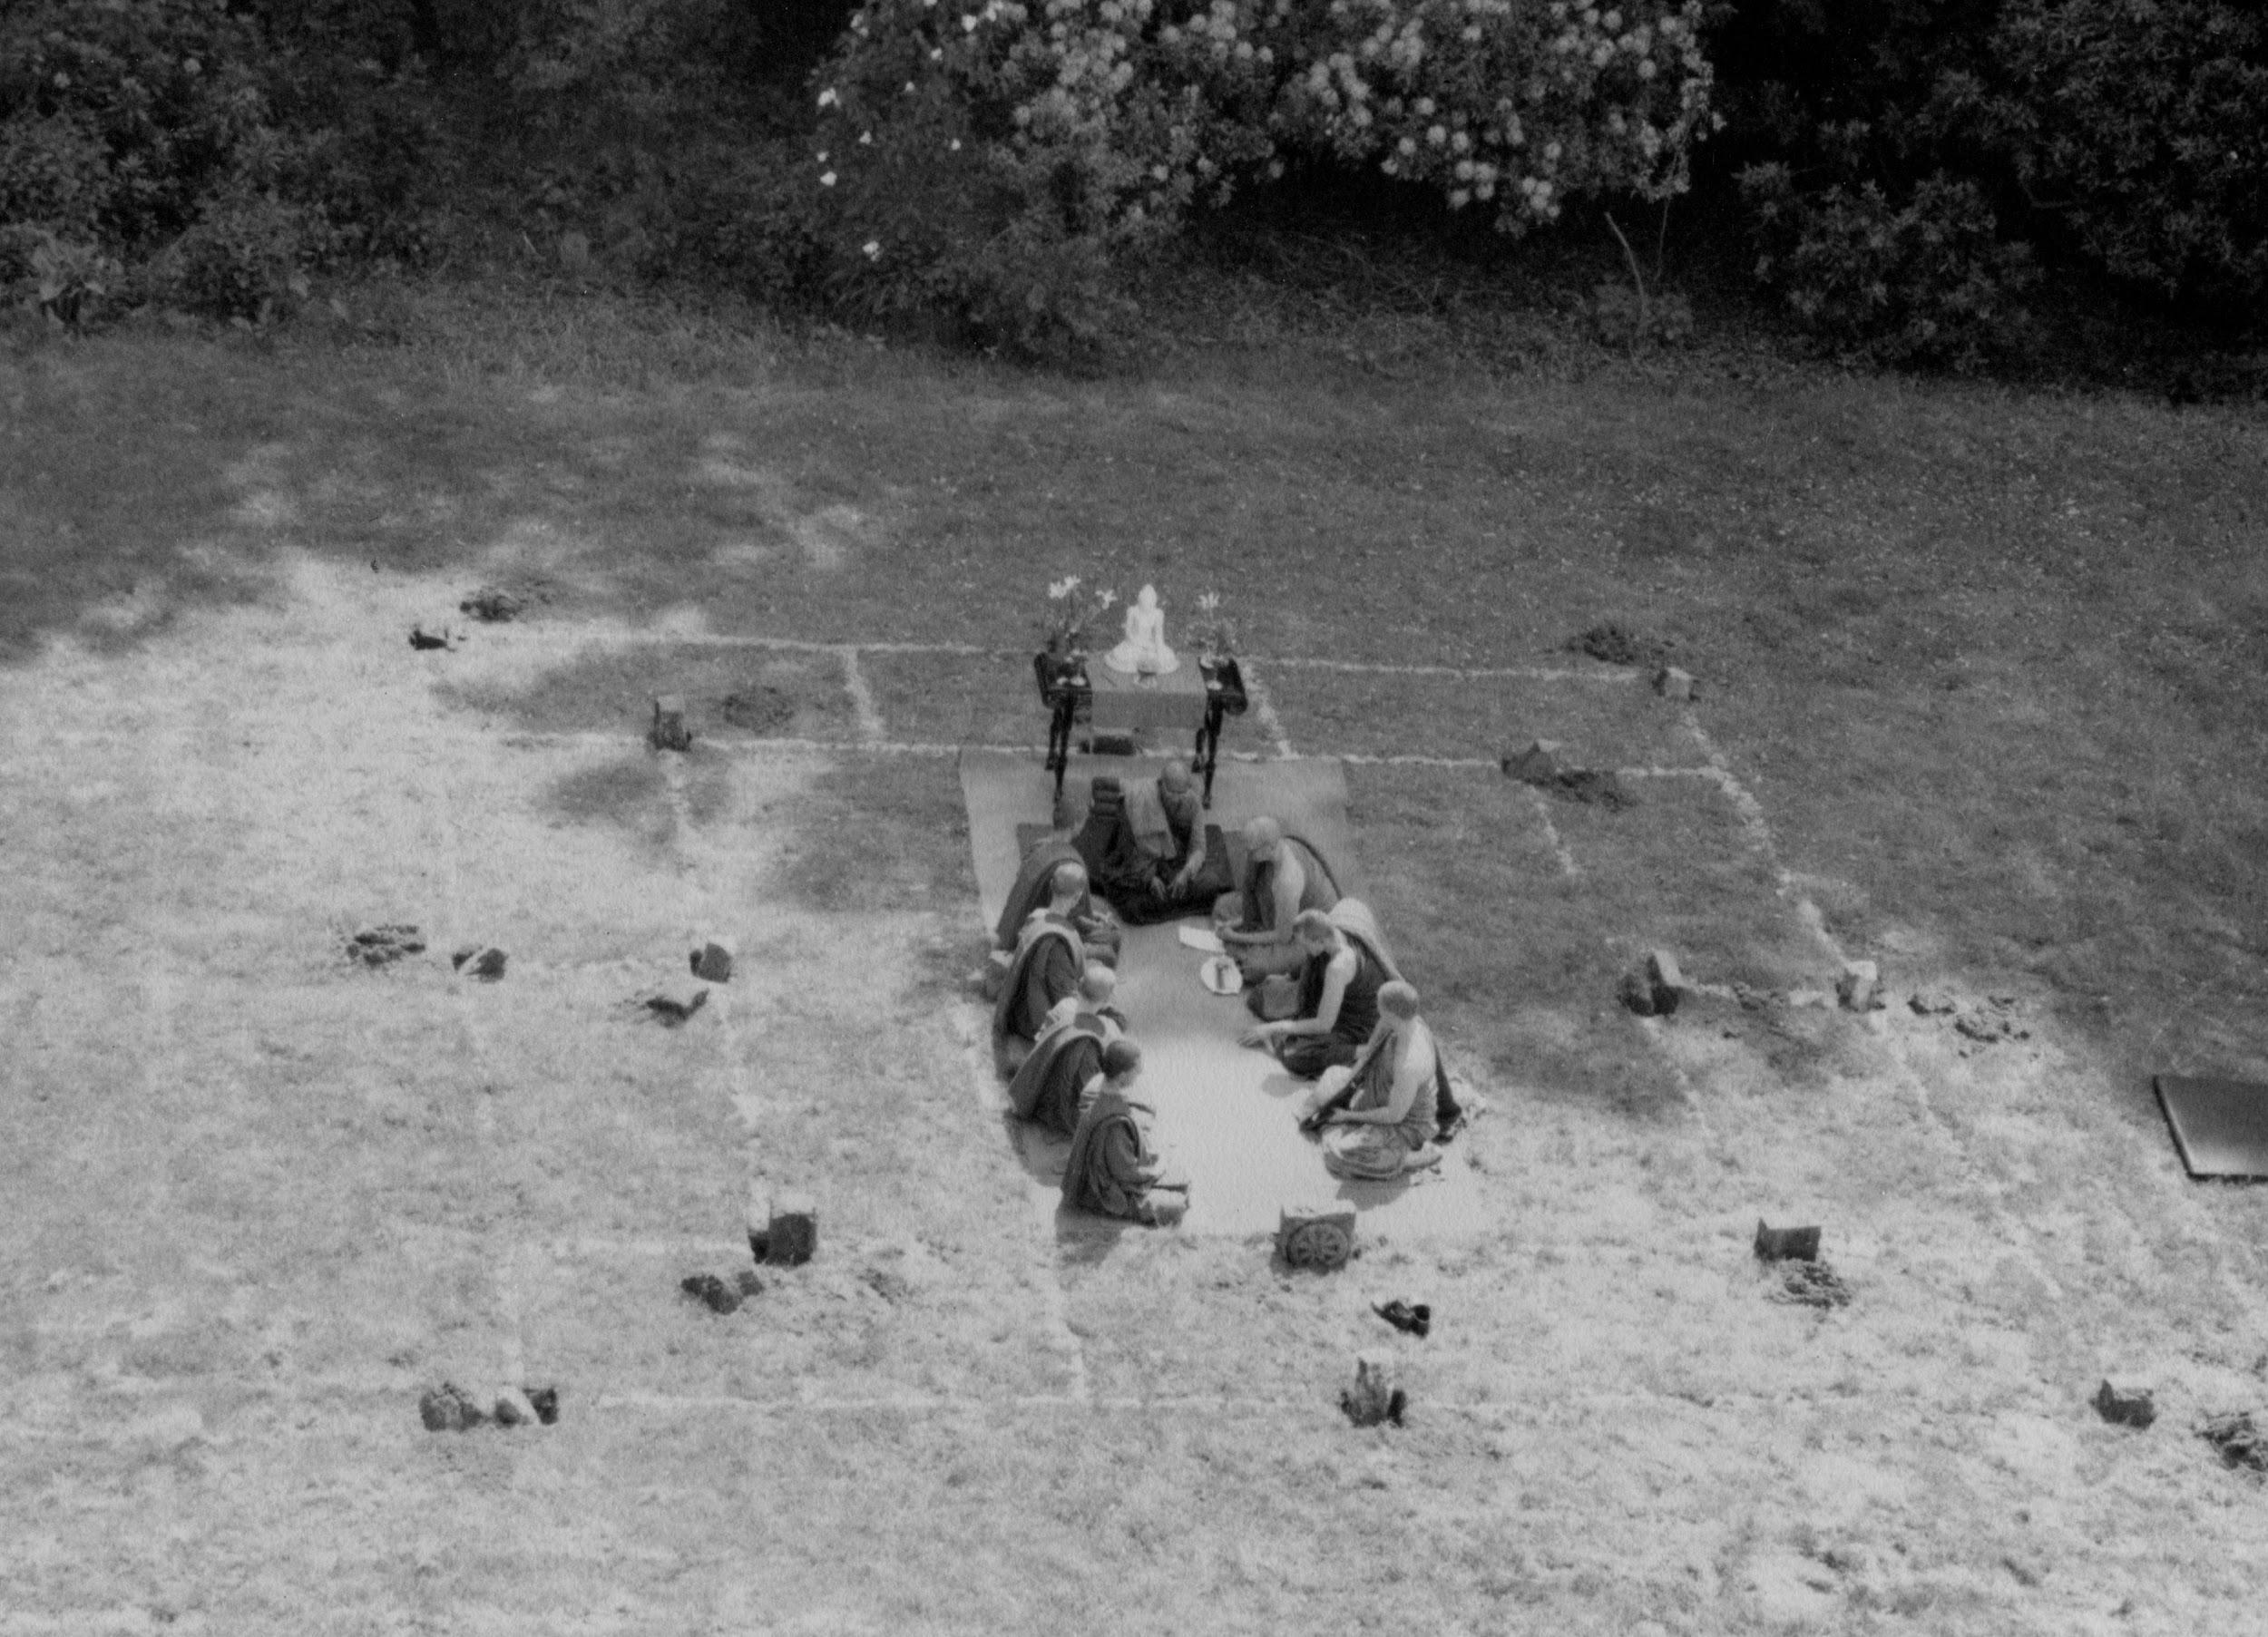
\includegraphics[width=\linewidth]{image6.jpeg}

When it came to the community feeling ready to establish a boundary\cite{sima}
at Chithurst, we had anticipated it would
require a lot of planning and preparation; we hoped that eventually we
would be able to create one out in the Hammer Wood. For Ven. Ananda
Maitreya, who had probably been involved in setting up many over the
years, there was nothing to it. In no time at all, we were out on the
old croquet lawn next to Chithurst House, going through the traditional
chanting: sorting out the possibility that there could have been an old
\emph{sima} boundary there before (from who knows when), and then
culminating in the formal procedure of declaring a new one. Once this
was properly established, the sangha at Chithurst was rightly prepared
to conduct Precept ceremonies. Indeed, for many years after that, this
was the place where all such ceremonies happened.

Bhante Dhammavara\cite{dhammavara} from Cambodia was another venerable Elder who
stayed with us a number of times in those early years. A good lay friend
of the sangha, who moved to live near the monastery, had spent time
training as a monk under Bhante Dhammavara in India. From him I later
learnt that Bhante became a monk around the age of thirty-three after
World War One had ended. Previously he had served as a district governor
and had a wife and a child. He lived as a monk for many years in India,
and a lot of his time was spent setting up and running a natural health
clinic. The first clinic was built in Northern India. After Partition\cite{partition},
it was deemed more suitable that he move to Delhi where, with
the help of Mrs Rameshwari Nehru\cite{nehru}, the wife of then
Prime Minister, Mr Nehru, he set up another
clinic. During his time staying with us at Chithurst, Bhante instructed
community members in ways of using colour for healing. Often this
involved drinking water that had been stored in coloured glass bottles.
For several years afterwards it was normal to come across coloured glass
bottles perched on windowsills around the monastery. In fact Bhante has
a significant repertoire of various skills that he had developed and
used over the years running those clinics in India.

Bhante Dhammavara was staying with us on the occasion that the
Ven. Maha Ghosananda\cite{ghosananda} came to visit. Also from Cambodia, Ven. Maha
Ghosananda had previously been the Supreme Patriarch in that country and
was renowned for his peace marches. When Ven. Maha Ghosananda passed
away in 2007, he was ninety-three years old. When Bhante Dhammavara
passed away in 1999, he was one hundred and ten.

The thing I remember about a visit by the Venerable Piyadassi Thera was
a comment he made during a talk he offered in which he summarized
practice by saying, `Just practise the Dhamma, leave the rest up to
kamma'. So simple that one might overlook its profundity. We easily make
practice complicated because of a lack of maturity in mindfulness,
restraint and wise reflection. Hearing these reminders from such
well-practised monks was significant.

There were also a number of inspiring female Dhamma teachers who
visited. During my time in Devon, Ajahn Sumedho had invited Dr.~Irmgard
Schloegl to use the gardens at Chithurst for her ordination. A retinue
of elders came over from Japan and performed the ceremony according to
their Rinzai Zen tradition, and Dr.~Irmgard Schloegl took on the name
Myokyo-Ni.

On one evening I recall seeing Ayya Khema\cite{khema}
at puja sitting in the midst of our Siladhara community. I
think our paths might have crossed some years earlier in Bangkok when
she was still Ilsa Liedermann. I do recall meeting her husband from back
then, Gert Liedermann, who spent time with us at Wat Pah Nanachat. He
was responsible for introducing the community to foot massage. Ilsa and
Gert had a property near Obi Obi in Queensland, Australia, where they
hosted Ajahn Khantipalo. Later on that property was sold and another
property in New South Wales was purchased, eventually to be known as Wat
Buddha Dhamma, where these days Ajahn Tiradhammo is living. Ayya Khema
went on to request Bhikshuni Precepts within the Mahayana tradition and
settled back in Germany, where she had been born, establishing a centre
called Buddha Haus\cite{buddha-haus}.

Ruth Dennison\cite{dennison}
also visited Chithurst in the early days. She was
one of the formally appointed teachers within the U Ba Khin meditation
tradition. As I recall, she stayed only briefly, but I was pleased some
years later to have a chance to visit her place, Dhamma Dena Vipassana
Center, out in the desert near Joshua Tree National Monument\cite{joshua}.

While reflecting on visits from venerable elders, I also want to
fast-forward a few years and mention the visit in 1990 from Master Hsuan
Hua. He brought with him a large group of his monks and nuns from
The City of Ten Thousand Buddhas\cite{ten-thousand}
in California. The venerable Master must have already
been very advanced in years, but his vitality was impressive, also his
generosity. His style of responding to questions was still very direct.
When one of our young monks who, at the time, was struggling in his
practice, asked a question hoping for some encouragement, Master Hua
told him that practice was like a tiger and it would eat you up. On
another occasion, when some of his monks and nuns asked if they could
learn our \emph{paritta} style of chanting, he scolded them saying they
were only interested in it because of the appealing tune, not because of
the Dharma content.

